\subsection{Optimisation dans les SGFD-R}
Ainsi, afin de mieux analyser les optimisations de la gestion de flux, il devient important d'investiguer plus en détail le fonctionnement de la gestion de base de données.

\subsubsection{Le problème dans sa globalité}
Le processus d'optimisation usuel en gestion de base de données est maintenant établie et répendue~\cite{Ioannidis:optimization}. Une requête en gestion de base de donnée est soumise par un langage déclaratif tel que \textit{SQL}. A partir de cette expression, s'enchaine une série d'opération qui permettra l'exécution de celle-ci. La figure \ref{fig:rw:sgfd:optim:processus} décrit le processus complet nécessaire à l'aboutissement de ce traîtement. 
\begin{figure}[h]
\centering
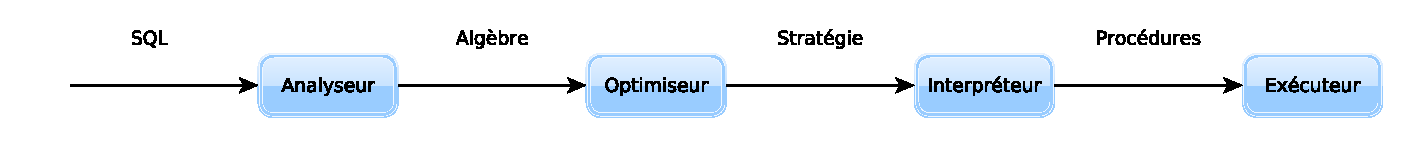
\includegraphics[width=0.9\textwidth]{rw-sgfd-optimsgbd}
\caption{Processus de traitement de requête dans un SGBD-R}\label{fig:rw:sgfd:optim:processus}
\end{figure}

Plusieurs modules permettent d'exécuter cette série d'opérations :
\begin{itemize}
   \item \textbf{Analyseur} : Prend en entrée une requête textuelle et fournit en sortie un arbre de requête écrit dans un format interne équivalent à de l'algèbre relationnelle. Ce module ne fait que traduire la grammaire du SQL par des règles prédéfinies.
   \item \textbf{Optimiseur} : Prend cet arbre de requête et fournit un autre arbre de requête, agrémenté d'indication de méthodes physique à utiliser. Le tout forme une stratégie d'exécution qui ne sera pas modifiée par la suite. Le but de cette étape est de fournir la stratégie qui fournit un résultat identique à ce que l'arbre initial était avec un coût moindre.
   \item \textbf{Interpréteur} : Récupère la stratégie d'exécution et instancie les procédures d'exécution. Le tout sera envoyé à l'\textbf{exécuteur} qui manipulera ces procédures afin de produire le résultat final.
\end{itemize}
L'optimiseur étant bien entendu le module le plus complexe car il possède et utilise beaucoup de connaissance et de résultats sur la gestion de données. Ce composant s'est prouvé indispensable dans la pratique car une bonne stratégie de traitement changera la plupart du temps de complexité ce qui transformera une requête pouvant être exécutée en plusieurs heures en moins d'une seconde.

Le problème est que l'espace des stratégies possibles pour exécuter une requête classique est potentiellement de cardinalité factorielle en fonction du nombre d'opérateurs et de méthodes d'exécutions disponibles (surtout s'il y a des jointures). Ainsi, il faut guider l'exploration et utiliser des techniques de programmation dynamique pour éliminer rapidement les branches trop coûteuses.

L'optimisation de requête se découpe en deux sections : l'optimisation logique (i.e. sélection du meilleur arbre d'opérateur théorique) et l'optimisation physique (choix des meilleurs algorithmes).

\subsubsection{Optimisation Logique}
L'espace algébrique est très large car les équivalences sur l'algèbre relationnelle sont très larges et permissives. Par exemple, une sélection sur une jointure $\sigma (R_1 \Join R_2)$ peut traverser l'opérateur binaire si sa condition ne concerne qu'une branche : $R_1 \Join \sigma R_2$. Ainsi, pour un arbre de requête, il peut y avoir des millions de requêtes équivalentes avec des permutations ou des ajouts d'opérateurs. Des heuristiques sont ainsi sélectionnées pour réduire cet espace tout en restant efficace~\cite{Ioannidis:optimization}. Le critère principal d'optimisation étant minimiser la taille des résultats intermédiaires. Voici les règles classiques :
\begin{itemize}
   \item[\textbf{R1}~:] \textit{La sélection et la projection n'introduisent pas de coût supplémentaires et sont traités à la volée}. Les sélections doivent être exécutés au moment de la première lecture sur la relation. Les projections doivent se faire en même temps que le résultat d'un autre opérateur.
   \item[\textbf{R2}~:] \textit{Les produits cartésiens ne doivent jamais être formés sauf si la requête elle-même en demande}. Seules les jointures peuvent combiner des relations.
   \item[\textbf{R3}~:] \textit{L'opérande interne (partie droite) de chaque jointure est une relation originelle, et non un résultat intermédiaire}.
\end{itemize}

La règle R1 est utilisée pour minimiser la taille des résultats intermédiaires. La règle R2 supprime toute possibilité de recours fatal aux algorithmes de boucles imbriquées sachant qu'un autre plan pouvait utiliser à chaque fois des jointures plus efficaces.

La règle R3 n'est pas toujours choisie car même si elle réduit beaucoup les possibilités car elle restreint les ordres de jointures, elle risque de supprimer l'arbre optimal dans plusieurs cas. En effet, les arbres de requêtes ne pourront pas être des arbres équilibrés car l'opérande droite doit être une relation native, or un arbre déséquilibré peut introduire des surcoûts du fait que les jointures supérieur doivent joindre une grande relation avec un résultat intermédiaire. Toutefois, il existe des raisons à cette règle. Tout d'abord, le fait d'avoir des relations natives permet l'utilisation d'index. De plus elle permet de faire un traitement total des requêtes en mode \textit{pipeline}\footnote{L'exécution en \textit{pipeline} permet de traiter un n-uplet dès sa lecture, notons que cela s'apparente à du traitement de flux. L'avantage étant que le processeur étant moins coûteux que les entrées-sorties, on peut rentabiliser l'attente de lecture en traitement de requête.}.

En parcourant l'espace algébrique des requêtes équivalentes vérifiant R1-3, le nombre de plans devient raisonnablement faible. Pour le reste des recherches, il sagit principalement de choisir l'ordre des jointures. Comme la jointure est symétrique $R_1 \Join R_2 = R_2 \Join R_1$ alors dans le cas de multiples jointures (courant en gestion de base de données), il faut choisir l'ordre le plus pertinent qui minimisera la taille des résultats intermédiaires. Cette recherche se fera conjointement avec l'optimisation physique du fait de son impact sur les algorithmes.

\subsubsection{Optimisation Physique}
L'optimisation physique correspond au parcours de l'espace des méthodes disponibles pour chaque plan de requête et à l'évaluation quantitative de chacune de celles-ci. L'espace des méthodes fournit plusieurs implémentation pour un opérateur. Par exemple pour la jointure :
\begin{itemize}
   \item \textbf{Boucles imbriqués} : Implémentation la plus directe de la jointure. Cet algorithme ne requiert aucune condition sur les relations d'entrées.
   \item \textbf{Jointure fusion} : Se base sur le fait que les deux relations sont triés sur l'attribut de jointure à l'avance. Ainsi la jointure est plus facile à effectuer. Elle est régulièrement utilisée avec des index triés comme les arbres B+~\cite{Comer:btree}. Des opérateurs de tri pourront être déployés si ces index sont absent.
   \item \textbf{Jointure hachée} : Se base sur le fait que les deux relations sont hachées sur l'attribut de jointure. Ainsi la jointure se fait sur les index de hachages de cardinalité réduite et d'accès rapide.
\end{itemize}

Pour chaque relation, il existe deux moyens principaux d'accéder à un n-uplet :
\begin{itemize}
\item \textbf{Scan} : Parcours strict de la relation ou d'un l'index pour trouver les n-uplets vérifiant une condition de sélection.
\item \textbf{Probe} : Demande directement aux procédures d'index de renvoyer les tuples vérifiant une condition de sélection.
\end{itemize}

Ainsi, il est possible de faire des boucles imbriqués suffisamment performantes en utilisant des accès optimisés aux relations. Bien évidemment certaines sélections sont impossibles via les procédures d'index. Par exemple, il est impossible de demander à un index haché de faire une sélection avec un opérateur de comparaison tel que \enquote{$\leq$}.

L'évaluation de chacune de ces méthodes passe par un coût global de l'exécution basé sur des statistiques. Ces statistiques aideront à quantifier la taille des résultats intermédiaires. Pour cela, il est nécessaire de faire des calculs de sélectivité~\cite{Selinger:selectivity}. Ces calculs permettent d'évaluer le ratio d'n-uplet qui valident une sélection. Par exemple, en l'absence d'information complémentaire, une sélectivité de 10\% est appliquée par défaut. Par la suite chaque algorithme est capable de quantifier son coût en fonction de ces sélectivités et des cardinalités des entités manipulées.

Suivant les capacités du système et la taille de la requête, le système pourra réordonner les jointures pour optimiser les algorithmes. La recherche dans cet espace de méthode se base sur la programmation dynamique. Elle permet de faire une recherche exhaustive sans être extrêmement coûteuse (par des procédures de \textit{branch \& bound} usuelles).

\paragraph*{Optimisation de la recherche}
La recherche exhaustive peut être très coûteuse si les jointures sont nombreuses car l'espace des stratégies devient large, ce qui peut être long à calculer. Une approche heuristique est nécessaire pour avoir un temps de calcul qui permette un lancement rapide de la requête. 

Plusieurs approches existent, la plus connue reste basée sur la marche aléatoire sur le graphe des stratégies possibles. Celle-ci parcourt le graphe aléatoirement en reculant si le coût est devenu trop important. Une autre approche intéressante étant l'utilisation d'algorithmes génétiques pour résoudre ce problème. \textit{Postgres} utilise l'optimiseur \textit{Genetic Query Optimizer (GEQO)}~\cite{Postgres:geqo} si le nombre de jointure dépasse une certaine limite.

L'optimisation a été prouvée comme un problème NP-complet~\cite{Ibaraki:join} (même avec seulement les boucles imbriqués) ainsi certains efforts se sont concentré sur la résolution de sous cas importants, notamment boucles imbriqués et jointure hachée seulement.

\paragraph*{Base de données parallèles}
L'optimisation en prenant en compte des modèles de calculs parallèles est un problème encore ouvert. Toutefois, des approximations efficaces se basent sur les optimisations à deux phases. Tout d'abord, le système recherche la solution optimale comme vu précédemment. Par la suite, il cherche le meilleur ordonnancement. Les deux domaines ont été suffisamment couverts pour obtenir des résultats satisfaisants.

\paragraph*{Distribution du calcul}
La distribution du calcul est un problème différent des bases parallèles dans le sens où il existe plusieurs unités d'évaluation complètement indépendantes. Le problème toutefois se résout principalement en quantifiant la distribution du calcul à l'intérieur de l'espace des méthodes. L'espace de recherche sera toutefois plus grand et il faudra faire attention à avoir un optimiseur performant pour ne pas avoir de surcoût avant l'exécution.

\paragraph*{L'optimisation sémantique}
Supposons la présence d'une base de connaissance en parallèle de la base de donnée. Il est alors possible de raisonner sur les conditions de sélections notamment, afin d'amener plus ou moins de restriction à la requête. Les calculs d'inférence de concepts, comme vus en section~\ref{sec:rw:supervision:contexte}, permettent d'extraire des conditions plus restrictives mais équivalentes. Le problème étant d'avoir une base de connaissance suffisamment exploitable car une erreur de raisonnement pourrait supprimer potentiellement des résultats. De plus, les calculs d'inférences peuvent être lourds et ne doivent pas rendre le traitement de requête trop lourd. Cette approche commence a être exploitée en gestion de flux de données aussi grâce à des méta-données~\cite{Ding:semantic}.
